% --------------------------------------------------------------
% This is all preamble stuff that you don't have to worry about.
% Head down to where it says "Start here"
% --------------------------------------------------------------

\documentclass[11pt,oneside]{article}

\usepackage[margin=1in]{geometry} 
\usepackage[spanish]{babel} 
\usepackage{color}
\usepackage{rotating}
\usepackage{fancybox}
\usepackage{lscape}
\usepackage{makecell}
\usepackage{graphicx}
\usepackage{ltablex}

\usepackage{booktabs}
\usepackage{multirow}

\usepackage{subcaption}
\usepackage[space]{grffile}
\usepackage[font=footnotesize,labelformat=simple]{subcaption}
\usepackage{float}
\usepackage{adjustbox}
\usepackage{graphicx}
\usepackage{threeparttable}
\usepackage{caption}
\usepackage{subcaption}
\usepackage{graphicx}
\usepackage{hyperref}
\usepackage[font=singlespacing]{caption}
\usepackage{longtable}
% Configuración de los márgenes
\geometry{
	left=3cm, % Margen izquierdo de 3 cm
	right=3cm, % Margen derecho de 3 cm
	top=2.5cm, % Margen superior de 2.5 cm
	bottom=2.5cm % Margen inferior de 2.5 cm
}


\usepackage{amsmath,amsthm,amssymb}
\newcommand{\code}{\texttt}
\newcommand{\N}{\mathbb{N}}
\newcommand{\Z}{\mathbb{Z}}
\newcommand{\E}{\mathbb{E}}


\newenvironment{theorem}[2][Theorem]{\begin{trivlist}
		\item[\hskip \labelsep {\bfseries #1}\hskip \labelsep {\bfseries #2.}]}{\end{trivlist}}
\newenvironment{lemma}[2][Lemma]{\begin{trivlist}
		\item[\hskip \labelsep {\bfseries #1}\hskip \labelsep {\bfseries #2.}]}{\end{trivlist}}
\newenvironment{exercise}[2][Exercise]{\begin{trivlist}
		\item[\hskip \labelsep {\bfseries #1}\hskip \labelsep {\bfseries #2.}]}{\end{trivlist}}
\newenvironment{problem}[2][Problem]{\begin{trivlist}
		\item[\hskip \labelsep {\bfseries #1}\hskip \labelsep {\bfseries #2.}]}{\end{trivlist}}
\newenvironment{question}[2][Question]{\begin{trivlist}
		\item[\hskip \labelsep {\bfseries #1}\hskip \labelsep {\bfseries #2.}]}{\end{trivlist}}
\newenvironment{corollary}[2][Corollary]{\begin{trivlist}
		\item[\hskip \labelsep {\bfseries #1}\hskip \labelsep {\bfseries #2.}]}{\end{trivlist}}

\newenvironment{solution}{\begin{proof}[Solution]}{\end{proof}}

% Load bibtex packages, including multibib to allow separate main paper \& appendix bibliographies.
\usepackage[round]{natbib}
\usepackage{authblk}
\usepackage{multibib}
\newcites{app}{Appendix References}


\begin{document}
	
	% --------------------------------------------------------------
	%                         Start here
	% --------------------------------------------------------------
	
	\title{Economía de la Distribución: Trabajo Práctico 2}
	\author{
		Emiliano Bohorquez \and 
		Brayan A. Condori Luque \and 
		Agustin Deniard}
	
	\maketitle
	
	%%%%%%%%%%%%%%%%%%%%%%%%%%%%%%%%%%%%%%%%%%%%%%%%%%%%%%%%%%%%%%%%%%%%%%%%
	% PREGUNTA 1
	%%%%%%%%%%%%%%%%%%%%%%%%%%%%%%%%%%%%%%%%%%%%%%%%%%%%%%%%%%%%%%%%%%%%%%%%
	\section*{Pregunta 1}
	
	
	%%%%%%%%%%%%%%%%%%%%%%%%%%%%%%%%%%%%%%%%%%%%%%%%%%%%%%%%%%%%%%%%%%%%%%%%
	% PREGUNTA 2
	%%%%%%%%%%%%%%%%%%%%%%%%%%%%%%%%%%%%%%%%%%%%%%%%%%%%%%%%%%%%%%%%%%%%%%%%
	\section*{Pregunta 2}
	
	
	%%%%%%%%%%%%%%%%%%%%%%%%%%%%%%%%%%%%%%%%%%%%%%%%%%%%%%%%%%%%%%%%%%%%%%%%
	% PREGUNTA 3 
	%%%%%%%%%%%%%%%%%%%%%%%%%%%%%%%%%%%%%%%%%%%%%%%%%%%%%%%%%%%%%%%%%%%%%%%%
	\section*{Pregunta 3}
	
	%%%%%%%%%%%%%%%%%%%%%%%%%%%%%%%%%%%%%%%%%%%%%%%%%%%%%%%%%%%%%%%%%%%%%%%%
	% PREGUNTA 4 
	%%%%%%%%%%%%%%%%%%%%%%%%%%%%%%%%%%%%%%%%%%%%%%%%%%%%%%%%%%%%%%%%%%%%%%%%
	\section*{Pregunta 4}

	\begin{figure}
    		\centering
    		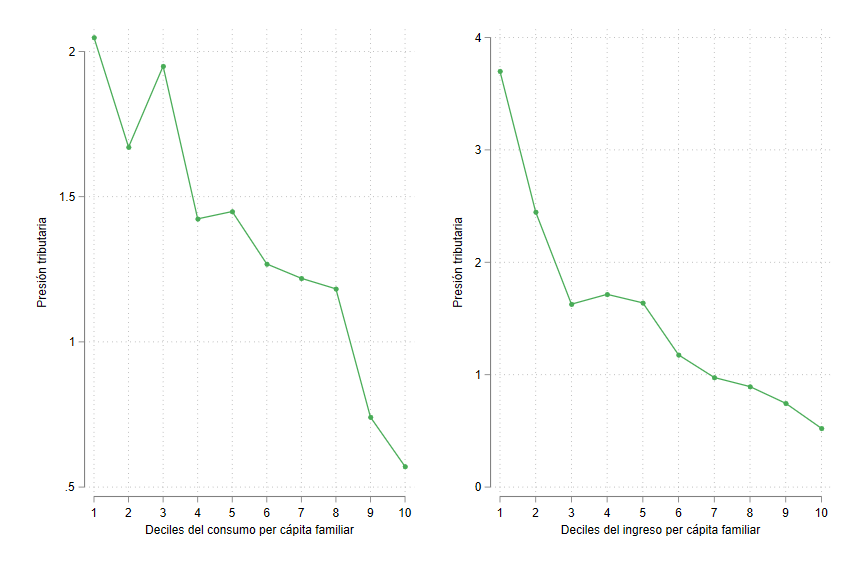
\includegraphics[width=1\linewidth]{presion_cigar.png}
    		\label{fig:4A}
	\end{figure}

	La figura \ref{fig:4A} refleja la presión que impone un impuesto a los cigarrillos sobre cada uno de los deciles de consumo (izquierda) y de ingreso (derecha) per cápita familiar. Podemos ver que, tomando como variable de interés tanto el consumo como el ingreso, la traslación total de la carga del impuesto a los consumidores termina por impactar de manera más fuerte sobre el consumo (ingreso) de los deciles más pobres de la distribución. 

	\begin{figure}
    		\centering
    		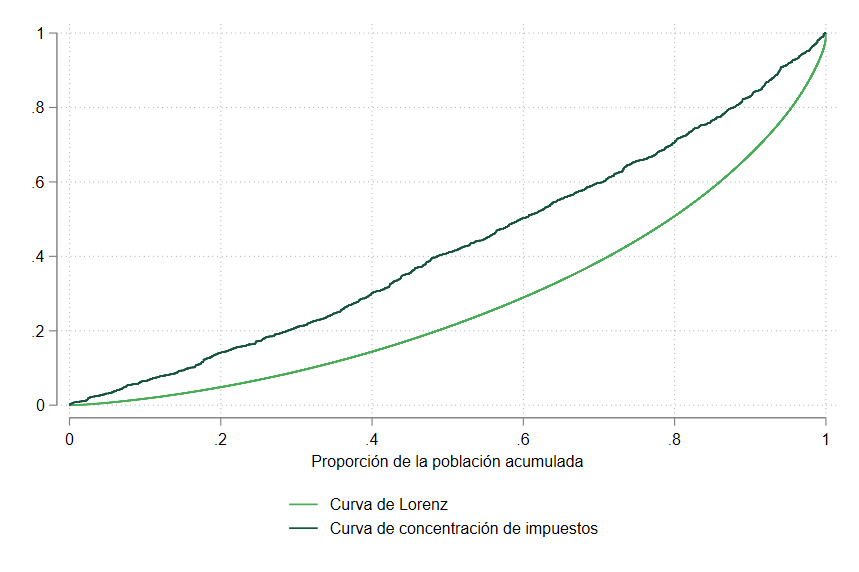
\includegraphics[width=0.75\linewidth]{concentracion_cigar.png}
    		\label{fig:4B}
	\end{figure}

	La figura \ref{fig:4B} presenta la curva de concentración del impuesto a los cigarrillos. El hecho de que la curva de concentración del impuesto se encuentre por encima de la curva de Lorenz nos informa que la carga del impuesto se distribuye de manera más ``igualitaria'' que el ingreso, lo cual implicaría que el impuesto a los cigarrillos tendría un efecto regresivo sobre la distribución del ingreso. Dado que el índice de Kakwani es igual a -0.2864, se confirma que el impuesto a los cigarrillos es un impuesto regresivo.
 
	%%%%%%%%%%%%%%%%%%%%%%%%%%%%%%%%%%%%%%%%%%%%%%%%%%%%%%%%%%%%%%%%%%%%%%%%
	% PREGUNTA 5
	%%%%%%%%%%%%%%%%%%%%%%%%%%%%%%%%%%%%%%%%%%%%%%%%%%%%%%%%%%%%%%%%%%%%%%%%
	\section*{Pregunta 5}
	%%%%%%%%%%%%%%%%%%%%%%%%%%%%%%%%%%%%%%%%%%%%%%%%%%%%%%%%%%%%%%%%%%%%%%%%
	% PREGUNTA 6
	%%%%%%%%%%%%%%%%%%%%%%%%%%%%%%%%%%%%%%%%%%%%%%%%%%%%%%%%%%%%%%%%%%%%%%%%
	\section*{Pregunta 7}
	%%%%%%%%%%%%%%%%%%%%%%%%%%%%%%%%%%%%%%%%%%%%%%%%%%%%%%%%%%%%%%%%%%%%%%%%
	% PREGUNTA 7
	%%%%%%%%%%%%%%%%%%%%%%%%%%%%%%%%%%%%%%%%%%%%%%%%%%%%%%%%%%%%%%%%%%%%%%%%
	\section*{Pregunta 7}
	
	
	
	
	
	% --------------------------------------------------------------
	%     You don't have to mess with anything below this line.
	% --------------------------------------------------------------
	%\newpage
	%\bibliographystyle{ecta}
	%\bibliography{references.bib}
	
	%\newpage
	%\appendix
	%\setcounter{table}{0}
	%\renewcommand{\tablename}{Cuadro Apéndice}
	%\renewcommand{\figurename}{Appendix Figure}
	%\renewcommand{\thetable}{A\arabic{table}}
	%\setcounter{figure}{0}
	%\renewcommand{\thefigure}{A\arabic{figure}}
	%%%%%%%%%%%%%%%%%%%%%%%%%%%%%%%%%%%%%%%%%%%%%%%%%
	
\end{document}

